\documentclass[border=8pt]{standalone}
\usepackage[T1]{fontenc}\usepackage[utf8]{inputenc}
\usepackage{helvet}\renewcommand{\familydefault}{\sfdefault}
\usepackage{tikz,xcolor}
\usetikzlibrary{arrows.meta,positioning,shapes.geometric,shapes.multipart,calc,fit,backgrounds,decorations.markings}
\definecolor{ink}{HTML}{1E1B16}\definecolor{paper}{HTML}{FBF8F2}\definecolor{clay}{HTML}{B5482A}\definecolor{soft}{HTML}{F1E9DA}\definecolor{pine}{HTML}{24402F}
\tikzset{
  every node/.style={font=\small,text=ink},
  >=Stealth, line/.style={draw=ink,line width=0.8pt},
  cls/.style={rectangle split,rectangle split parts=3,draw=ink,line width=0.8pt,fill=soft,align=left,inner xsep=6pt,inner ysep=4pt,
              rectangle split part align={center,left,left},minimum width=3.0cm},
  cls2/.style={rectangle split,rectangle split parts=2,draw=ink,line width=0.8pt,fill=soft,align=left,inner xsep=6pt,inner ysep=4pt,
              rectangle split part align={center,left},minimum width=3.0cm},
  box/.style={rectangle,draw=ink,line width=0.8pt,fill=soft,align=center,inner sep=5pt,minimum height=0.8cm},
  state/.style={rectangle,rounded corners=8pt,draw=ink,line width=0.8pt,fill=soft,align=center,inner sep=6pt,minimum width=2.2cm,minimum height=0.9cm},
  act/.style={rectangle,rounded corners=10pt,draw=ink,line width=0.8pt,fill=soft,align=center,inner sep=5pt,minimum width=2.4cm,minimum height=0.8cm},
  dec/.style={diamond,draw=ink,line width=0.8pt,fill=soft,inner sep=1pt,minimum width=0.9cm,minimum height=0.9cm},
  uc/.style={ellipse,draw=ink,line width=0.8pt,fill=soft,align=center,inner sep=3pt,minimum width=3.2cm,minimum height=1.0cm},
  note/.style={rectangle,draw=ink,line width=0.6pt,fill=yellow!12,align=left,inner sep=4pt,font=\footnotesize},
  lab/.style={font=\footnotesize,fill=paper,inner sep=1.5pt},
  err/.style={},
}
\newcommand{\actor}[3]{% x,y,label
  \draw[line width=0.8pt] (#1,#2+0.55) circle (0.17);
  \draw[line width=0.8pt] (#1,#2+0.38)--(#1,#2-0.15) (#1-0.3,#2+0.22)--(#1+0.3,#2+0.22) (#1,#2-0.15)--(#1-0.25,#2-0.6) (#1,#2-0.15)--(#1+0.25,#2-0.6);
  \node[font=\small] at (#1,#2-0.9) {#3};}
\begin{document}
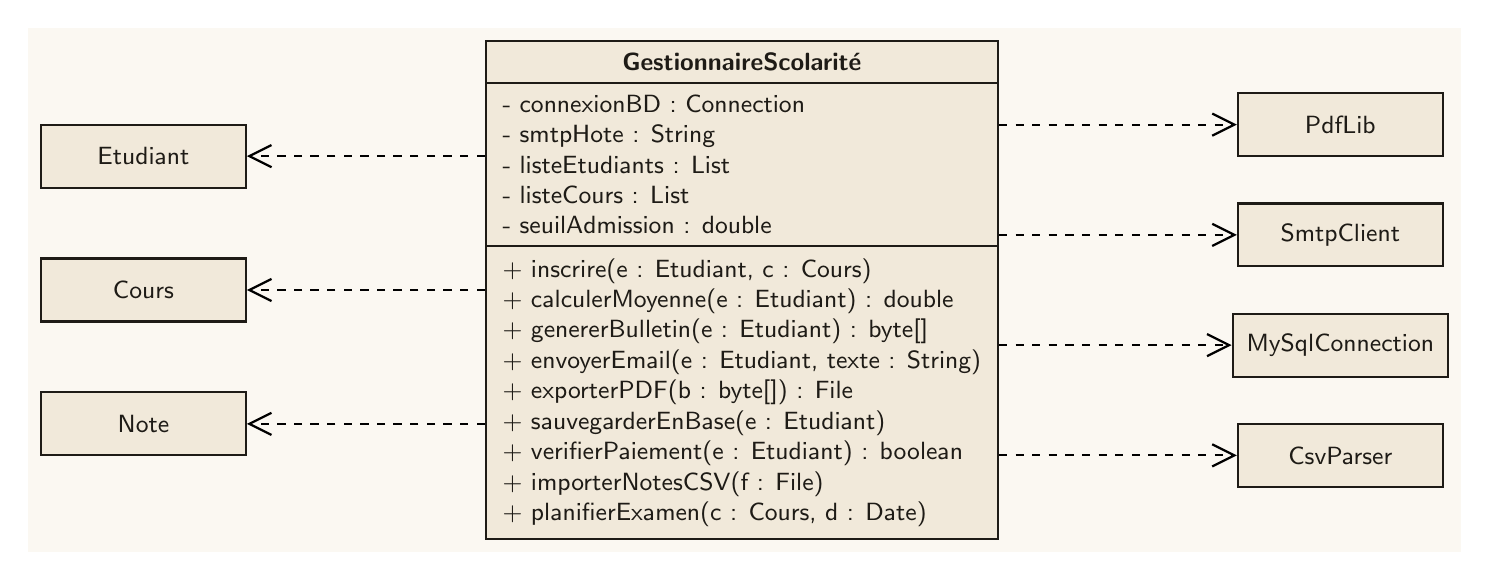
\begin{tikzpicture}[background rectangle/.style={fill=paper},show background rectangle]
\node[cls,minimum width=6.4cm,anchor=center] (g) at (0,0) {\textbf{GestionnaireScolarité}\nodepart{two}- connexionBD : Connection\\- smtpHote : String\\- listeEtudiants : List\\- listeCours : List\\- seuilAdmission : double\nodepart{three}+ inscrire(e : Etudiant, c : Cours)\\+ calculerMoyenne(e : Etudiant) : double\\+ genererBulletin(e : Etudiant) : byte[]\\+ envoyerEmail(e : Etudiant, texte : String)\\+ exporterPDF(b : byte[]) : File\\+ sauvegarderEnBase(e : Etudiant)\\+ verifierPaiement(e : Etudiant) : boolean\\+ importerNotesCSV(f : File)\\+ planifierExamen(c : Cours, d : Date)};
\node[box,minimum width=2.6cm] (n0) at (-7.6,1.7) {Etudiant};
\draw[dashed,line width=0.8pt,-{Straight Barb[length=8pt,width=8pt]}] (g.west |- n0.east) -- (n0.east);
\node[box,minimum width=2.6cm] (n1) at (-7.6,0.0) {Cours};
\draw[dashed,line width=0.8pt,-{Straight Barb[length=8pt,width=8pt]}] (g.west |- n1.east) -- (n1.east);
\node[box,minimum width=2.6cm] (n2) at (-7.6,-1.7) {Note};
\draw[dashed,line width=0.8pt,-{Straight Barb[length=8pt,width=8pt]}] (g.west |- n2.east) -- (n2.east);
\node[box,minimum width=2.6cm] (n3) at (7.6,2.1) {PdfLib};
\draw[dashed,line width=0.8pt,-{Straight Barb[length=8pt,width=8pt]}] (g.east |- n3.west) -- (n3.west);
\node[box,minimum width=2.6cm] (n4) at (7.6,0.7) {SmtpClient};
\draw[dashed,line width=0.8pt,-{Straight Barb[length=8pt,width=8pt]}] (g.east |- n4.west) -- (n4.west);
\node[box,minimum width=2.6cm] (n5) at (7.6,-0.7) {MySqlConnection};
\draw[dashed,line width=0.8pt,-{Straight Barb[length=8pt,width=8pt]}] (g.east |- n5.west) -- (n5.west);
\node[box,minimum width=2.6cm] (n6) at (7.6,-2.1) {CsvParser};
\draw[dashed,line width=0.8pt,-{Straight Barb[length=8pt,width=8pt]}] (g.east |- n6.west) -- (n6.west);
\end{tikzpicture}
\end{document}
